% Chapter 5

\chapter{Adversarial Networks Training} % Main chapter title
\label{Chapter5} % For referencing the chapter elsewhere, use \ref{Chapter1} 

Now that we built our dataset, we have the data we need to proceed with the adversarial training of our pipeline.

It is once again important to place this chapter in the context of our data pipeline, as we introduced it in section~\ref{sec:datapipeline} and as we showed it in figure~\ref{fig:pipeline}. The dataset we just created is composed of policies (which are just tables or 2D matrices).  More specifically we have 3,827 such policies, corresponding to all the 3,827 different valid map configurations of our environment, \code{RandomisedFrozenLake}. We split the dataset in a training subset (80\%) of the total number of policies, and the test subset (the remaining 20\%).

In section~\ref{sec:gan} we introduced Generative Adversarial Networks, detailing their vanilla architecture, as they were introduced by \citeauthor{goodfellow2014generative}. We now build off of this architecture to build a GAN architecture for policy generation.

In this section we present such architecture, explain the design decisions that were involved in configuring it, and describe the process of training it in an adversarial manner. We also provide a detailed breakdown of the generator and the discriminator's deep neural networks. We also make our Keras implementation of our Policy GAN publicly available.

The input to our Policy GAN will only be the training subset of the policies we trained with Q-learning. In this way, we hope to be able to model, through our GAN, a distribution on these policies such that we can capture knowledge that we can transfer to other unseen tasks.
These unseen tasks are exactly the ones corresponding to the map configurations of the test subset, and we therefore do not include those test policies as our input to our GAN.

%----------------------------------------------------------------------------------------

\section{Policy GAN}
In figure~\ref{fig:PolicyGAN} we show the architecture of our Policy GAN.
We already described most of the details involved when training GANs in section~\ref{sec:gan}. 

Training a GAN is an iterative process that runs for a set amount of epochs (an epoch is one full training cycle on the training set).
At each iteration, the mini-batch inputs to the discriminator \code{D} are taken from both the real data sampled from the training data (in our case policies from the training set that we created in chapter~\ref{Chapter4}), and the samples generated by the generator.
Given \code{D}'s prediction, we then apply a gradient-based optimisation method to update both \code{D}'s and \code{G}'s parameters.

Building neural net architecture that work well in practice generally involves finding and tuning many parameters and making several design decisions that make the issue not trivial. In the following subsections, we introduce such decisions and hyperparameters choice with the aim of allowing reproducibility of our results.

As we can notice, the Generator network outputs a vector of size dimension 64, which we can then reshape to a 16x4 matrix. This is our 'fake', generated Q-table. Its input is just a the latent space vector $z$ of size 100 whose values we can set randomly. We can interpret $z$ as a noise vector which deterministically influences the Q-table that we generate. While we can vary $z$ and obtain different Q-tables, these generated Q-tables should still fall within the initial distributions of Q-tables we have in our dataset, provided that the Generator was trained properly.

The Discriminator network, in turn, takes in an input a vector of size 64 (which is a reshaped 16x4 Q-table), and outputs a single scalar in $[0,1]$ representing the predicted probability that the inputted Q-table is a generated policy or one sampled from the dataset.


\begin{figure}
\centering
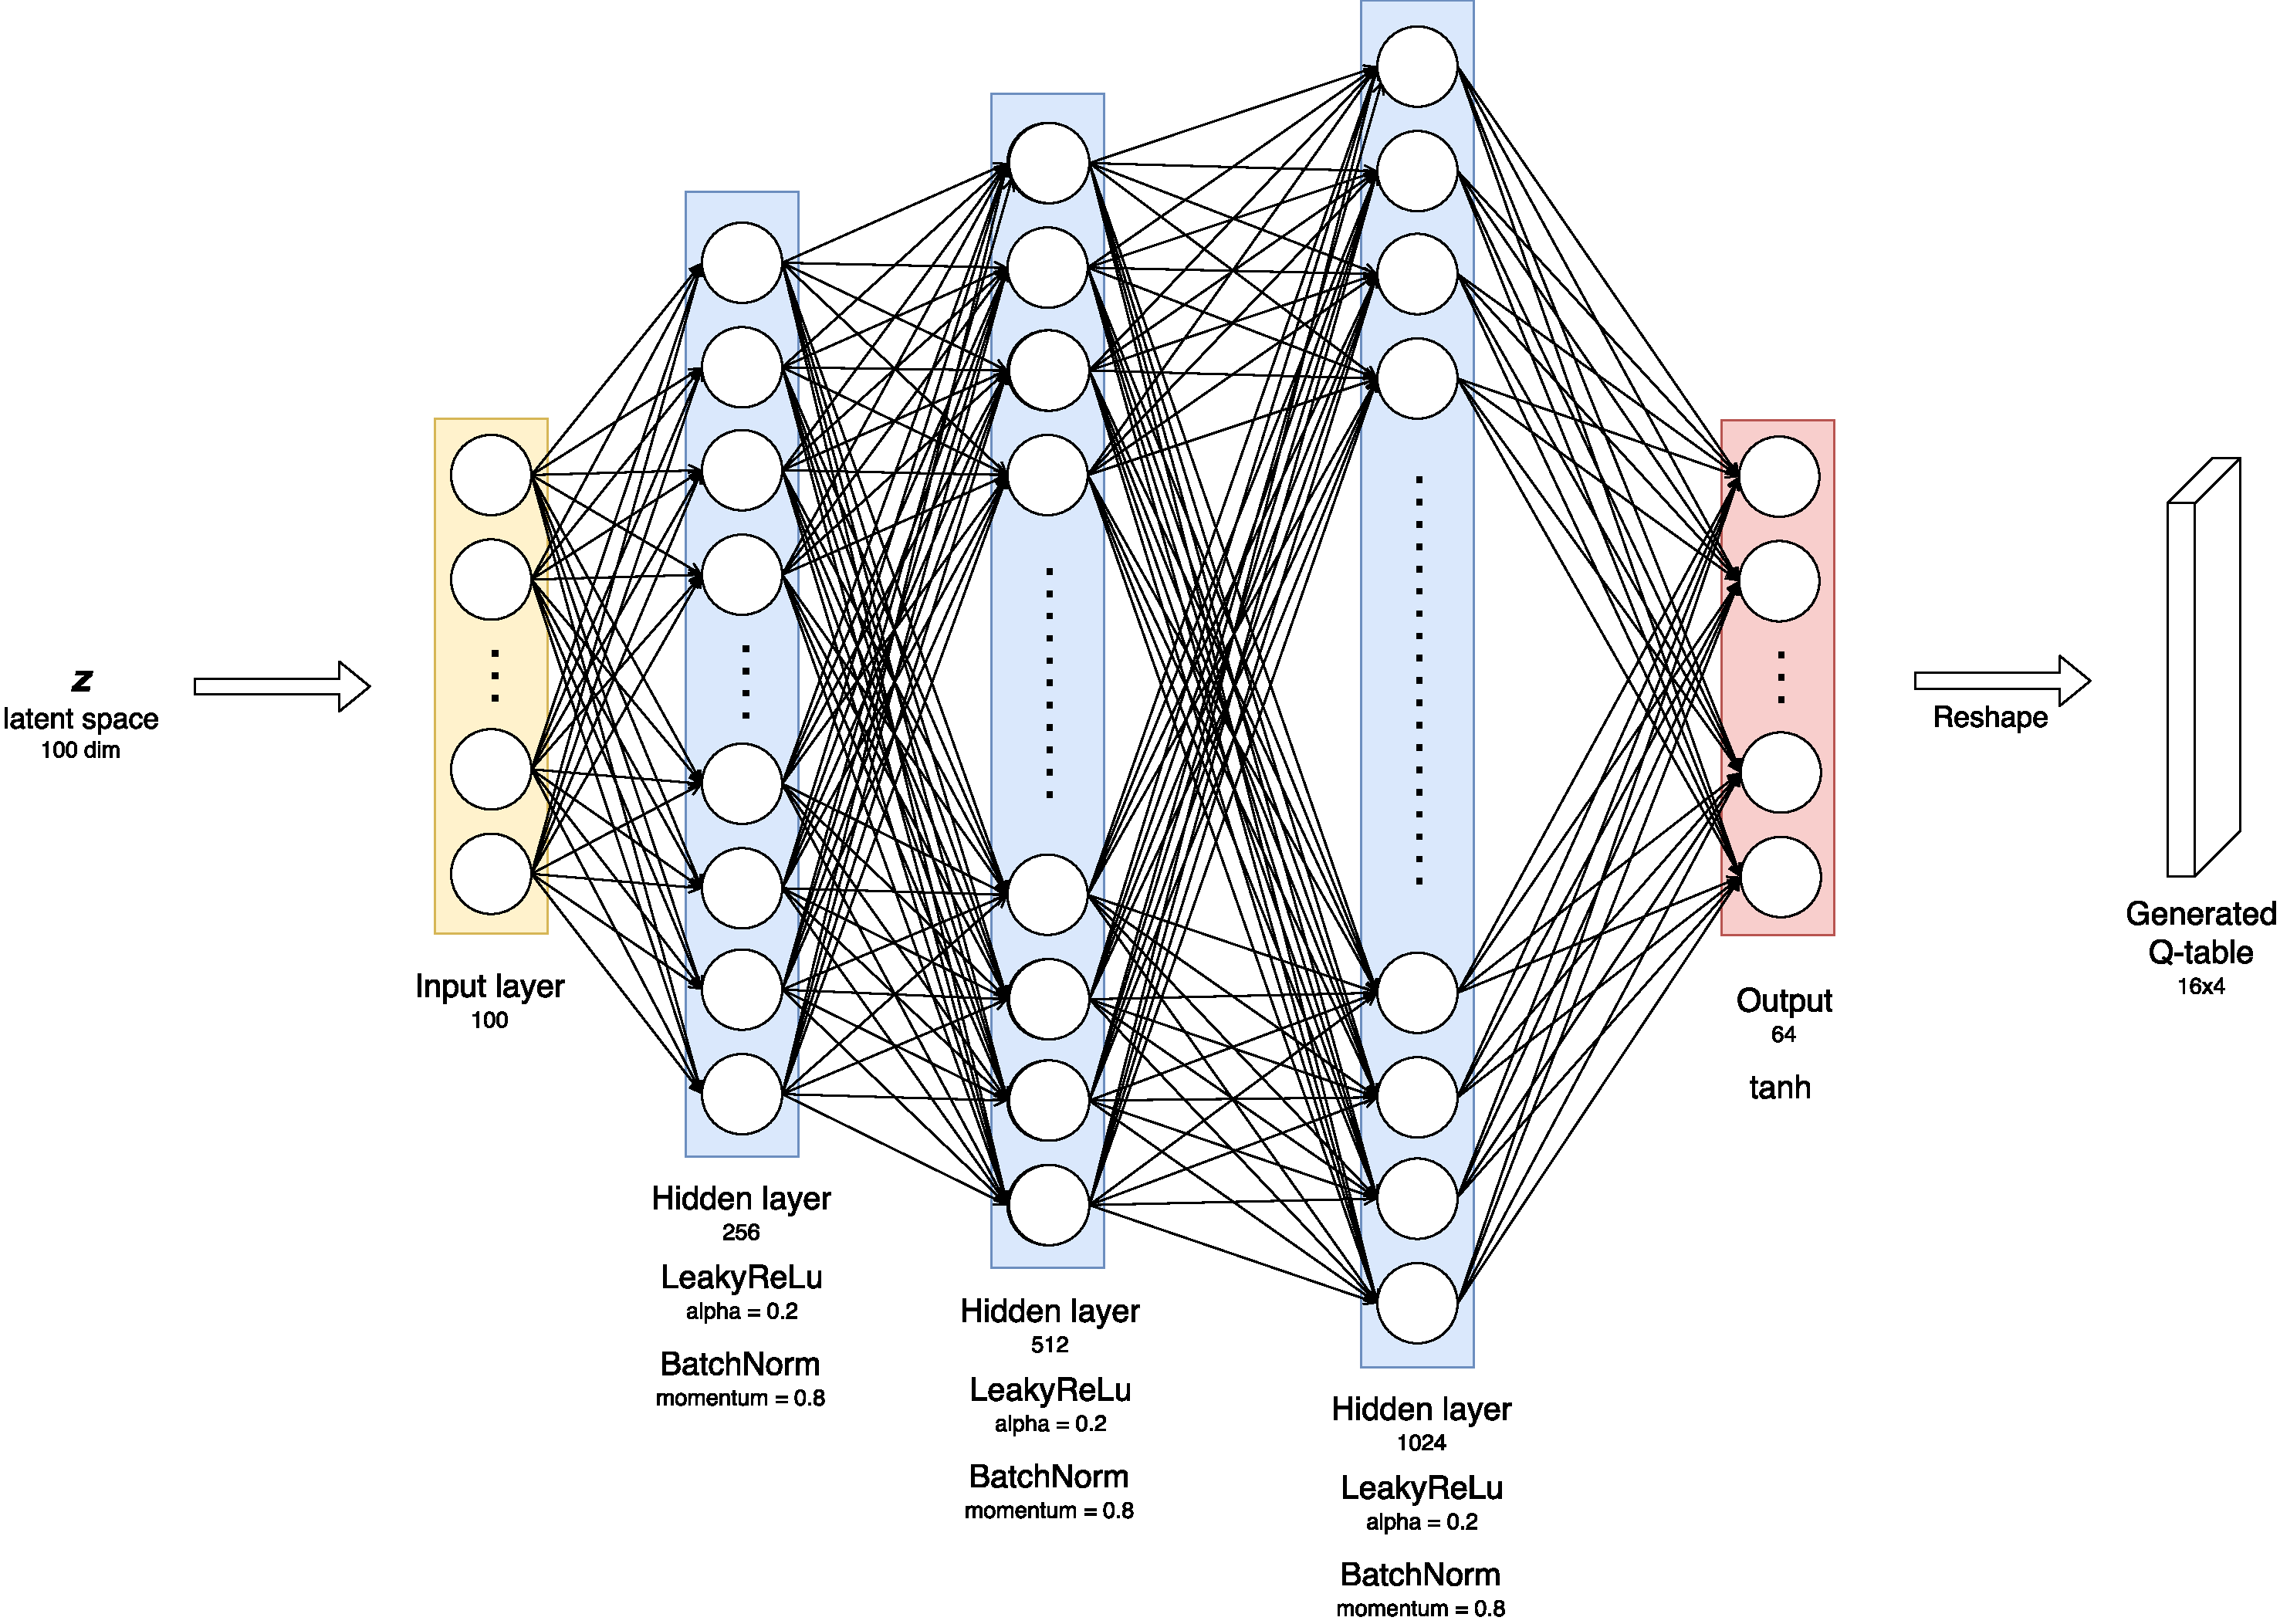
\includegraphics[width=15cm]{Figures/Generator}
\caption{Architecture of the Generator network}
\label{fig:Generator}

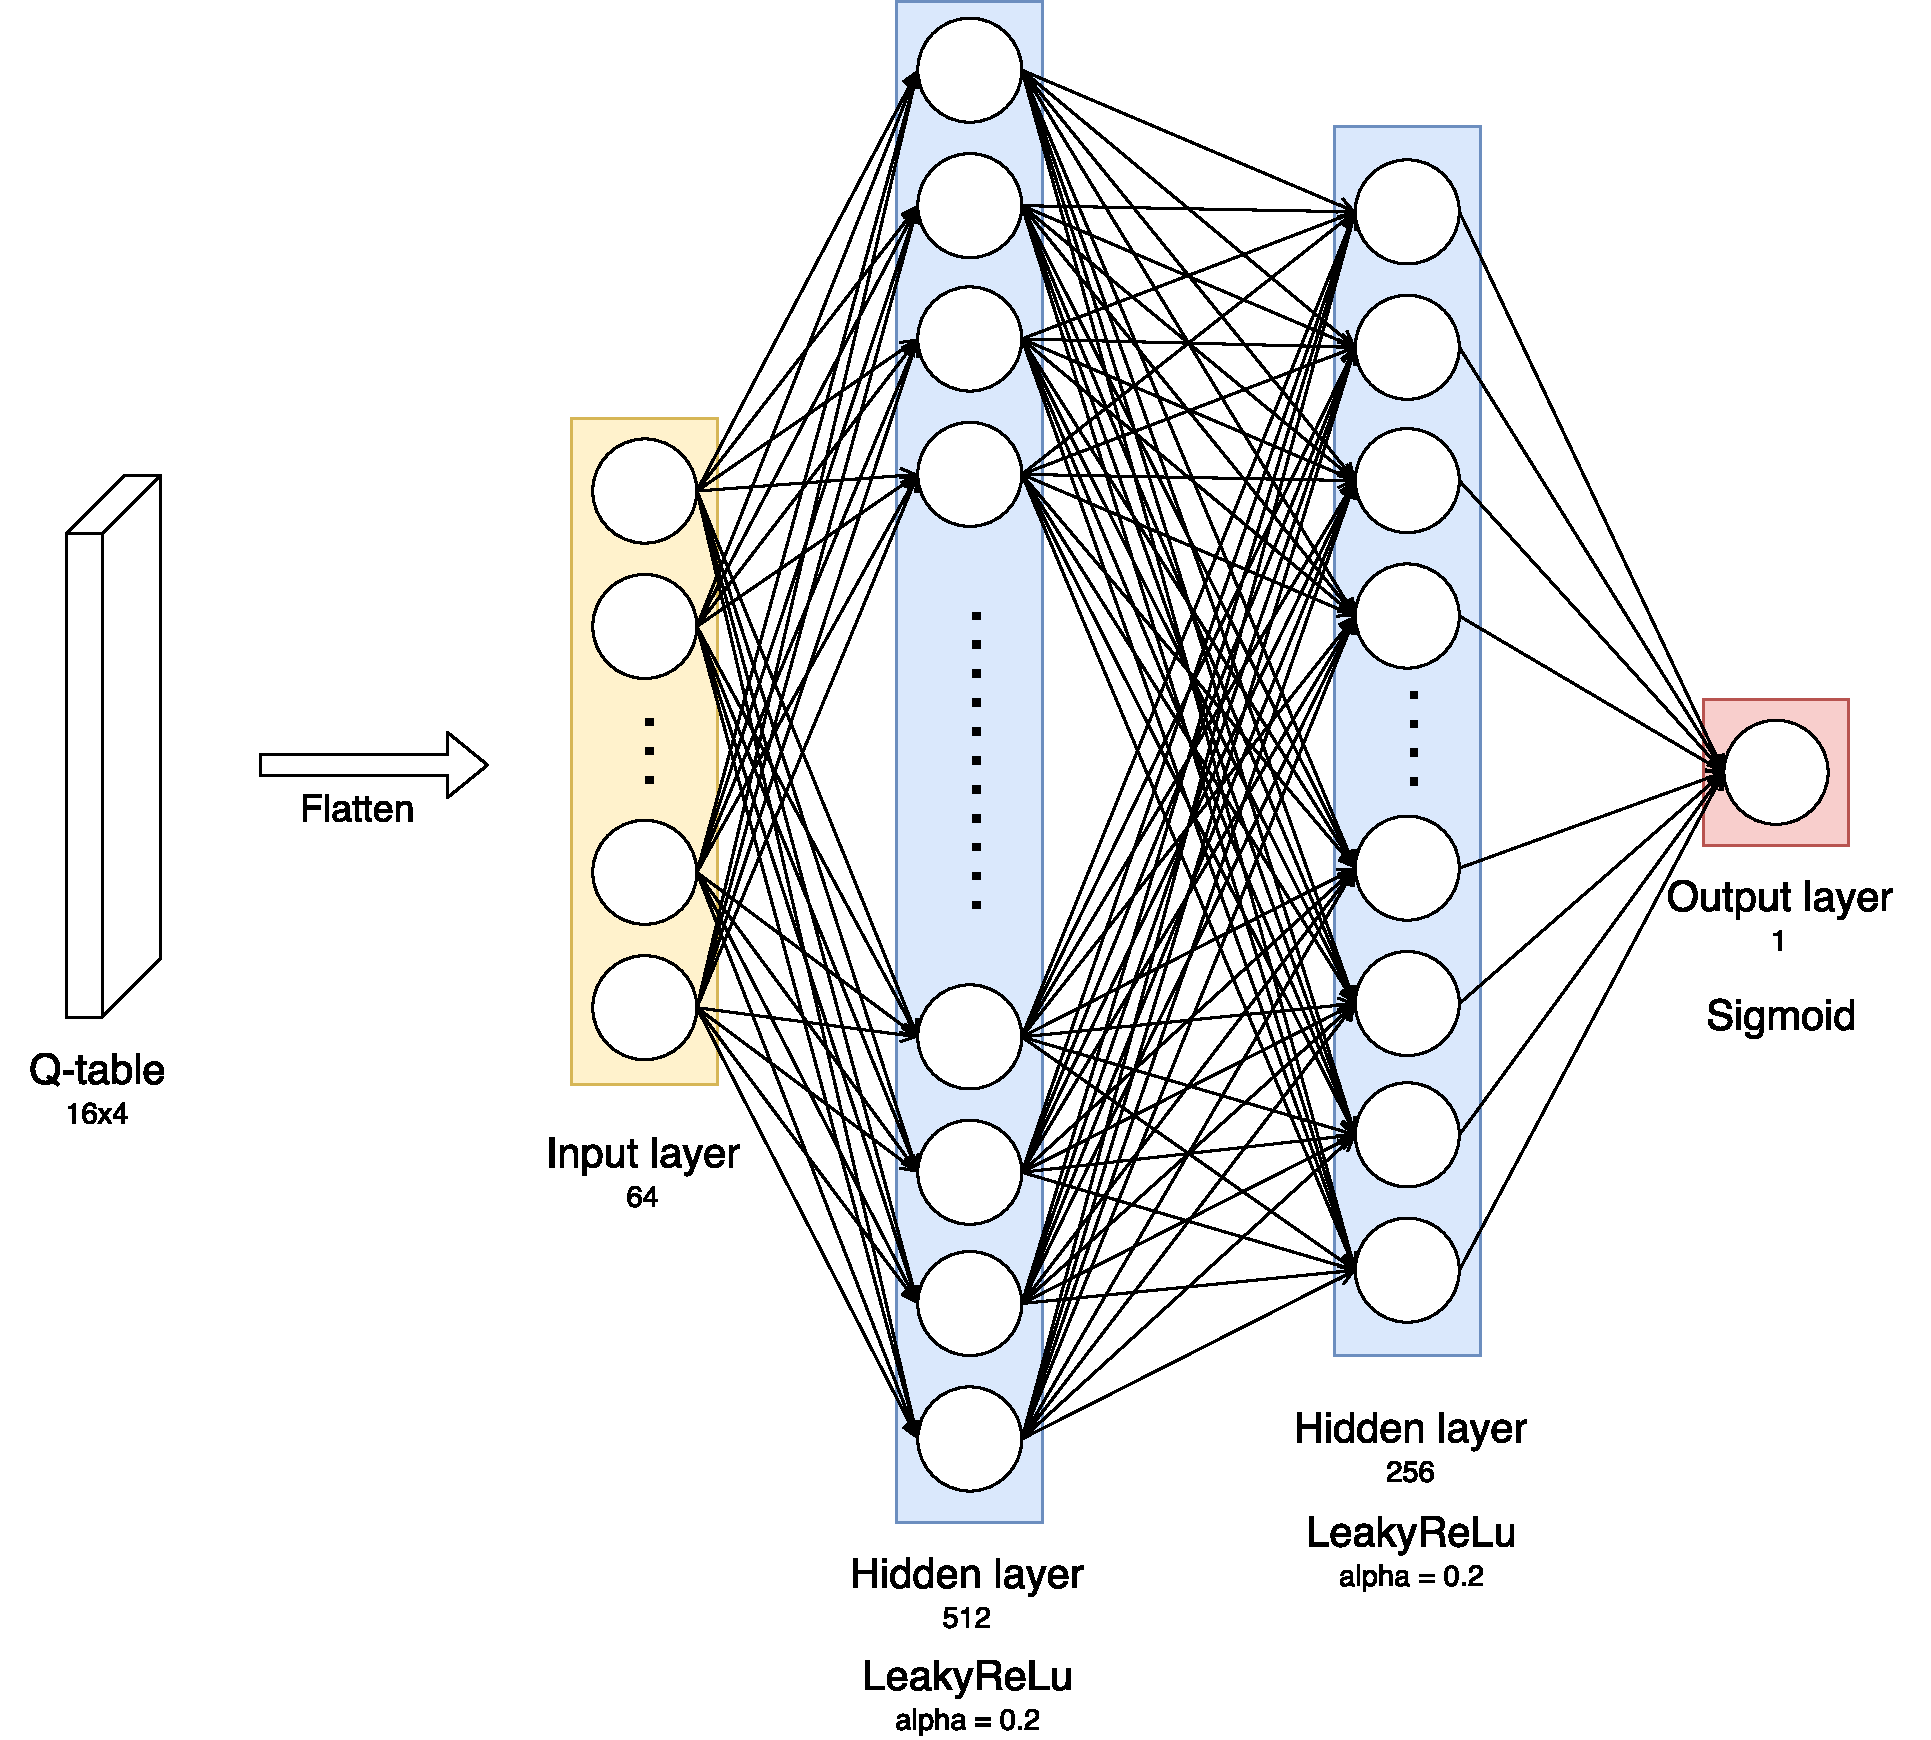
\includegraphics[width=10cm]{Figures/Discriminator}
\caption{Architecture of the Discriminator network}
\label{fig:Discriminator}
\end{figure}


\begin{figure}
\centering
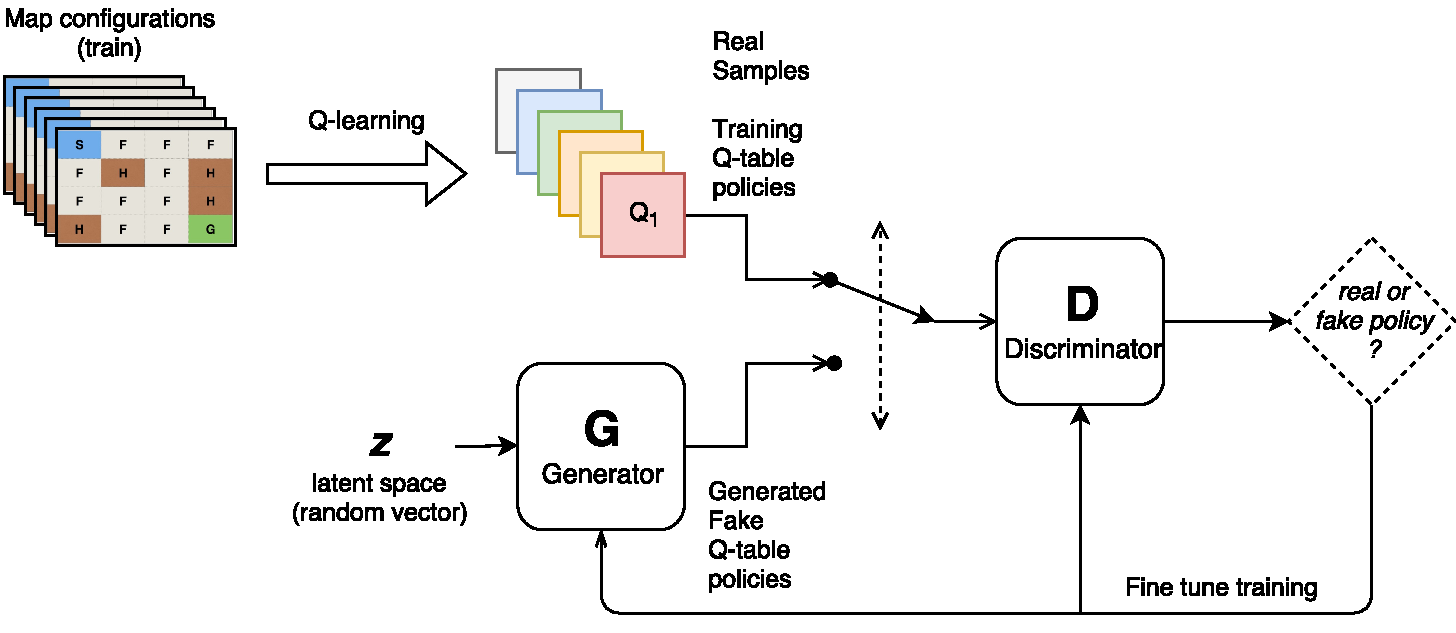
\includegraphics[width=15cm]{Figures/PolicyGAN}
\caption{Our Policy GAN architecture}
\label{fig:PolicyGAN}
\end{figure}

\subsection{Gradient descent optimisation}
Learning rates and gradient descent optimisations algorithms have historically been among the trickiest hyperparameters to set, as they drastically influence the final results, perhaps more than all other hyperparameters.

Gradient descent \citep{lemarechal2012cauchy}, a seminal approach to optimisation that dates back to Cauchy a few centuries back, still proves relatively successful in many machine learning applications.
Since then, a lot of work has been put in devising algorithms that have adaptive learning rates and that lead to faster convergence. In our design, we specifically explored two such adaptive learning rates algorithms: RMSProp \citep{hinton2012neural} and Adam \citep{DBLP:journals/corr/KingmaB14}

Both perform local optimisation with different techniques and metrics that are constructed from the history of previous interactions.

RMSProp (algorithm \ref{alg:RMSProp}) is a modification of the AdaGrad optimiser \citep{duchi2011adaptive}, that modifies the gradient accumulation into a moving average that is exponentially weighted.

Adam (algorithm \ref{alg:Adam}) is best described as a combination of RMSProp and Stochastic Gradient Descent (SGD) with momentum \citep{sutskever2013importance}. Momentum accelerates SGD by multiplying the learning rate by a parameter that increases as we go towards the right direction in the gradient update.

\begin{algorithm}[ht]
\begin{algorithmic}
   \State {\bfseries Require:} Global learning rate $\epsilon$, decay rate $\rho$
   \State {\bfseries Require:} Initial parameter $\theta$
   \State {\bfseries Require:} Small constant $\delta$, usually $10^{-6}$, used to stabilize division by small number
   
   \State Initialize accumulation variables $\boldsymbol{r=0}$
   \While{stopping criterion not met}{}
   \State Sample a minibatch of $m$ examples from the training set $\{x^{(1)},...,x^{(m)}\}$ with corresponding targets $y^{i}$.
   \State Compute gradient: $\boldsymbol{g \leftarrow \frac{1}{m}\nabla_\theta \sum_i L(f(x^{(i)}; \theta), y^{(i)}).}$
   \State Accumulate squared gradient: \\ $\boldsymbol{r \leftarrow \rho r + (1 - \rho) g \odot g}$
   \State Compute parameter update: $\boldsymbol{\Delta\theta = -\frac{\epsilon}{\sqrt{\delta+r}} \odot g.}$ ($\frac{1}{\sqrt{\delta+r}}$ applied element-wise)
   \State Apply update: $\boldsymbol{\theta \leftarrow \theta + \Delta \theta}$
   \EndWhile
\end{algorithmic}
  \caption{RMSProp algorithm}
  \label{alg:RMSProp}
\end{algorithm}


\begin{algorithm}[ht]
\begin{algorithmic}
   \State {\bfseries Require:} Step size $\epsilon$ (Suggested default: 0.001)
   \State {\bfseries Require:} Exponential decay rates for moment estimates, $\rho_1$ and $\rho_2$ in $[0,1)$. (Suggested defaults: 0.9 and 0.999 respectively)
   \State {\bfseries Require:} Small constant $\delta$ used for numerical stabilisation (Suggested default: $10^{-8}$)
   \State {\bfseries Require:} Initial parameters $\theta$
   
   \State Initialise 1st and 2nd moment variables $\mathbf{s=0, r=0}$
   \State Initialise time step $t=0$
   \While{stopping criterion not met}{}
   \State Sample a minibatch of $m$ examples from the training set $\{x^{(1)},...,x^{(m)}\}$ with corresponding targets $y^{i}$.
   \State Compute gradient: $\boldsymbol{g \leftarrow \frac{1}{m}\nabla_\theta \sum_i L(f(x^{(i)}; \theta), y^{(i)}).}$
   \State $t \leftarrow t + 1$
   \State Update biased first moment estimate: $\boldsymbol{s \leftarrow \rho_1 s + (1-\rho_1) g}$
   \State Update biased second moment estimate: $\boldsymbol{r \leftarrow \rho_2 r + (1-\rho_2) g \odot g}$
   \State Correct bias in first moment: $\boldsymbol{\hat{s} \leftarrow \frac{s}{1-\rho_1^t}}$
   \State Correct bias in second moment: $\boldsymbol{\hat{r} \leftarrow \frac{r}{1-\rho_2^t}}$
   \State Compute update: $\boldsymbol{\Delta \theta = -\epsilon \frac{\hat{s}}{\sqrt{\hat{r}} + \delta}}$
   \State Apply update: $\boldsymbol{\theta \leftarrow \theta + \Delta \theta}$
   \EndWhile
\end{algorithmic}
  \caption{Adam algorithm}
  \label{alg:Adam}
\end{algorithm}

Like in most applications involving deep learning, there is no definite way to see which approach would yield the best results without going through the whole training process.

We therefore empirically experiment with each of these approaches to see which choice is more suitable to our data distribution and yields the best results.

"Best", in our case, is seen in the context of both the Generator network and the Discriminator network. We look for an optimisation technique that leads to stable costs for both networks. In most deep learning problems, convergence of the cost function is limited to one single neural network. In adversarial architectures like GANs, or architectures with multiple deep neural networks like Variational Autoencoders (VAE), or Actor-Critic networks, convergence of the model is not a property that we can evaluate as trivially \citep{kingma2013auto, grondman2012survey}.

We look for an asymptotic behaviour that has both networks converge to an optimum, without having one network prevail over the other. For example, we could have a Discriminator that produces perfect predictions after a few epochs of training, but that is a meaningless result if the Generator is not able to produce results that can "fool" the discriminative model.

The overall cost of the architecture, in short, must take into account both components. The cost of the whole architecture has the following closed form:
\[\min_{G} \max_{D} V(G, D) = \mathbb{E}_{x\sim p_{data}(x)}[log D(x)] + \mathbb{E}_{z \sim p_{g}(z)}[log(1-D(G(z)))] \]

With both RMSProp and Adam, we obtain a much better convergence compared to vanilla SGD. While we do not notice a noticeable difference between these two results, having adaptive learning rates clearly helps convergence for both models.

After optimising our hyperparameters with grid-search, our final optimal optimisation algorithm is the following: \\
Adam, step size $\epsilon = 0.0002$, exponential decay rates $\rho_1 = 0.5$, $\rho_2 = 0.999$.

%TODO Comparisons of design decisions graphs


%----------------------------------------------------------------------------------------

\subsection{Activation functions}
Another important design decision when building neural networks pertains to the choice of activation function we use in our hidden layers.

In the context of neural network training, an activation function $\varphi$ is one that we apply to the outputs of hidden layers, i.e. $\varphi(y)$ where $y=W^Tx + b$.

What makes activation functions so critical is the fact that they allow us to model non-linear data distributions, enabling us to build more complex representations of our predictions.

Historically, non-linear activations functions like the logistic sigmoid function or tanh function, while successful with certain data distributions, have proven difficult to train, mostly due to their non-zero centered property and slope of the function \citep{DBLP:journals/corr/XuHL16}.
Many activations functions have been introduced in machine learning literature, with some working well with many practical applications.

In this section, we provide an overview of such activation functions, all of which we evaluated in our GAN training experiments.

We trained different Policy GAN models using different combinations of activations functions for the Generator and the Discriminator's hidden layers. The activation we accounted for were the following: sigmoid function, ReLU function (Rectified Linear Unit) \citep{DBLP:journals/corr/AroraBMM16}, Leaky ReLU \citep{DBLP:journals/corr/XuWCL15}, ELU or Exponential Linear Units \citep{DBLP:journals/corr/ClevertUH15}, and SELU or Scaled Exponential Linear Units \citep{DBLP:journals/corr/KlambauerUMH17}.

Following are the definitions of the considered activations functions with their respective gradients, followed, in figure~\ref{fig:activationfns}, by a their visualisation on the x-y axis.\\

\textbf{Sigmoid}:
\begin{flalign}
  \text{sigmoid}(x) = \frac{1}{1+\exp{-x}}
\end{flalign}

\textbf{ReLU}:
\begin{flalign}
  \text{relu}(x) = \max(0, x)
\end{flalign} 

\textbf{Leaky ReLU:}
\begin{flalign}
  \text{lrelu}(x) = 
  \begin{cases} 
      \alpha x      & \quad \text{if } x \leq  0 \\
      x       & \quad \text{if } x > 0 .
    \end{cases} 
\end{flalign} 

\textbf{ELU:}
\begin{equation}
  \text{elu}(x) = 
  \begin{cases} 
      \alpha (\exp(x) - 1)      & \quad \text{if } x \leq  0 \\
      x       & \quad \text{if } x > 0 .
    \end{cases} 
\end{equation} 

\textbf{SELU:}
\begin{equation}
  \text{selu}(x) = \lambda
  \begin{cases} 
      \alpha (\exp(x) - 1)      & \quad \text{if } x \leq  0 \\
      x       & \quad \text{if } x > 0 .
    \end{cases} 
\end{equation} 

\begin{figure}
\vskip -3mm
\begin{center}
\centerline{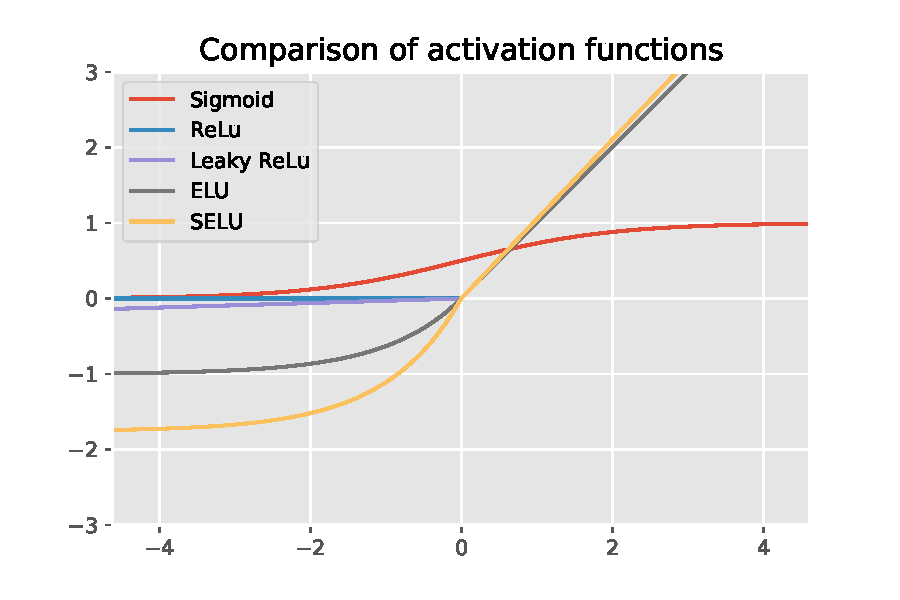
\includegraphics[width=10cm]{Figures/ActivationFns}}
\caption{Plots of activation functions}
\label{fig:activationfns}
\end{center}
\vskip -3mm
\end{figure}
As we expected, different activations functions yield varying degree of successful results, with Leaky ReLu ($\alpha=0.2$) producing the best overall results for both the Generator and the Discriminator model.

Using all other activations functions in our hidden layer, with the exception of the sigmoid function, yield good results.
The sigmoid activation function model likely incurred incurred into the vanishing gradient problem \citep{DBLP:journals/corr/abs-1211-5063}, where a big amount of possible inputs are 'squashed' into a relatively small range (0, 1). Other activation functions like LeakyReLu, ELU or SELU address this problem by giving a wider range of continuous values for negative inputs.

While the use of the sigmoid function as activation for the hidden layers creates this issue, it is still greatly functional to model a binary classification problem. More specifically, the Discriminator network, which is effectively a binary classifier determining whether the input is 'fake' or 'real', can still make use of a sigmoid activation in its output layer to model the probability of the input being real.

\subsection{Weight initialisation}
A common easy approach to weight initialisation is to use small random values as weights, most commonly sample from a normal distribution $N\sim \mathcal{N}(0, \sigma)$. Having a 'smarter' weight initialisation, however, may lead to  faster convergence when training our models.

One such approach is using sampling from the following uniform distribution:

\begin{equation}
 W \sim U(-\frac{1}{\sqrt{n_{in}}}, \frac{1}{\sqrt{n_{in}}})
\end{equation}

where $n_{in}$ is the number of incoming connections of each unit in the hidden layer.

Another, slightly more sophisticated approach to weight initialisation is the Glorot/Xavier initilisation \citep{pmlr-v9-glorot10a}, whereby weights are sampled from the following uniform distribution:

\begin{equation}
W \sim U\Bigg(-\sqrt{\frac{6}{n_{in}+n_{out}}}, \sqrt{\frac{6}{n_{in}+n_{out}}}\Bigg)
\end{equation}

where, once again, $n_{in}$ is the number of incoming connections of each neuron in the hidden layer. Similarly, $n_{out}$ is the number of outgoing connections.

We experimented will all these three variations to initialise the weights in our neural network. Since there is randomness involved in these techniques, we ran the GAN training multiple times. On average, Glorot/Xavier initialisation led to 6\% fewer epochs required before both the generator and the discriminator converged.

\subsection{Batch Normalisation}
Batch Normalisation \citep{DBLP:journals/corr/IoffeS15} is a technique that improves stability and performance of neural networks by normalising the inputs of each layer such that they have a mean output activation of zero and standard deviation of one. Benefits of using batch normalisation include faster training time (i.e. faster convergence to optimal model). This also allows higher learning rates and and makes weight initialisation not as critical.

We first compute the mean and variance of each hidden unit activation across the minibatch (size $M$):
\begin{gather*}
\mu_i \leftarrow \frac{1}{M} \sum_{m=1}^{M}u_i^m \\
\sigma_i^2 \leftarrow \frac{1}{M} \sum_{m=1}^{M}(u_i^m - \mu_i)^2
\end{gather*}

The result of doing batch normalisation will then be:
\begin{gather*}
u_i = w_ix \\
\hat{u_i} = \frac{u_i-\mu_i}{\sqrt{\sigma_i^2 + \epsilon}} \\
z_i = \gamma_i\hat{u_i}+\beta_i = \text{batchNorm}({u_i})
\end{gather*}

where $\gamma$ and $\beta$ are parameters updated with gradient descent that will scale and shift the normalised activations.

We trained two different models for both the Generator and the Discriminator models: one with Batch Normalisation and one without, keeping the rest of the architecture and hyperparameter settings fixed.
Using Batch Normalisation in the Generator network leads to much faster convergence than the model that does not make use of it.
The Discriminator network, effectively being a much less complex model than the Generator, did not benefit from batch-normalised inputs in terms of speed of model convergence and overall cost.

\section{Final architecture and results}
%TODO: Couple of words on task generalisation + move architectures here
We report here the architectures of final optimal deep neural networks for the Generator model and the Discriminator model. Figure~\ref{fig:Generator} and figure~\ref{fig:Discriminator} show a visualisation for the two networks respectively.\\\\
\textbf{Generator}:
\begin{itemize}[noitemsep]
	\item Input: 100 dim
	\item Hidden Layer 1: 256 dim
	\begin{itemize}[noitemsep,topsep=0pt]
		\item Activation: LeakyReLu(alpha = 0.2)
		\item BatchNormalisation(momentum = 0.8)
	\end{itemize}
	\item Hidden Layer 2: 512 dim
	\begin{itemize}[noitemsep,topsep=0pt]
		\item Activation: LeakyReLu(alpha = 0.2)
		\item BatchNormalisation(momentum = 0.8)
	\end{itemize}
		\item Hidden Layer 3: 1024 dim
	\begin{itemize}[noitemsep,topsep=0pt]
		\item Activation: LeakyReLu(alpha = 0.2)
		\item BatchNormalisation(momentum = 0.8)
	\end{itemize}
	\item Output Layer: 64 dim
	\begin{itemize}[noitemsep,topsep=0pt]
		\item Activation: tanh
	\end{itemize}
\end{itemize}
\phantom\\
\textbf{Discriminator}:
\begin{itemize}[noitemsep]
	\item Input: 64 dim
	\item Hidden Layer 1: 512 dim
	\begin{itemize}[noitemsep,topsep=0pt]
		\item Activation: LeakyReLu(alpha = 0.2)
	\end{itemize}
	\item Hidden Layer 2: 256 dim
	\begin{itemize}[noitemsep,topsep=0pt]
		\item Activation: LeakyReLu(alpha = 0.2)
	\end{itemize}
	\item Output Layer: 1 dim
	\begin{itemize}[noitemsep,topsep=0pt]
		\item Activation: sigmoid
	\end{itemize}
\end{itemize}

Let us look at the convergence of both networks. We plot the losses of both Generator and Discriminator in figure~\ref{fig:GANLosses}. The graph on the left reports the actual values for both losses. Since these tend to oscillate greatly during training (as it is typical with gradient-based optimisations), we also provide a version smoothed with IIR filtering, on the right. We notice that both losses asymptotically converge after around 1,000 epochs of training.

Initially, we observe that the Discriminator's loss (in blue) hovers just around 0. That is due to the fact that the Generator was not properly trained yet (notice the its high losses in orange). In early epochs, the Generator is likely producing unrealistic policies that the Discriminator is easily able to discern.

However, as we train the Generator a few more epochs, the policies that it produces tend to fit the initial distribution of policies more, which make its loss decrease, and the Discriminator loss increase slightly. Both then converge after a few more hundred epochs, at around epoch 1,000.

It takes the Generator more epochs to train since it is a neural network with much higher complexity (one additional hidden layer, and more hidden units). This explains the trend of both losses that the figure reports.

\begin{figure}
\centering
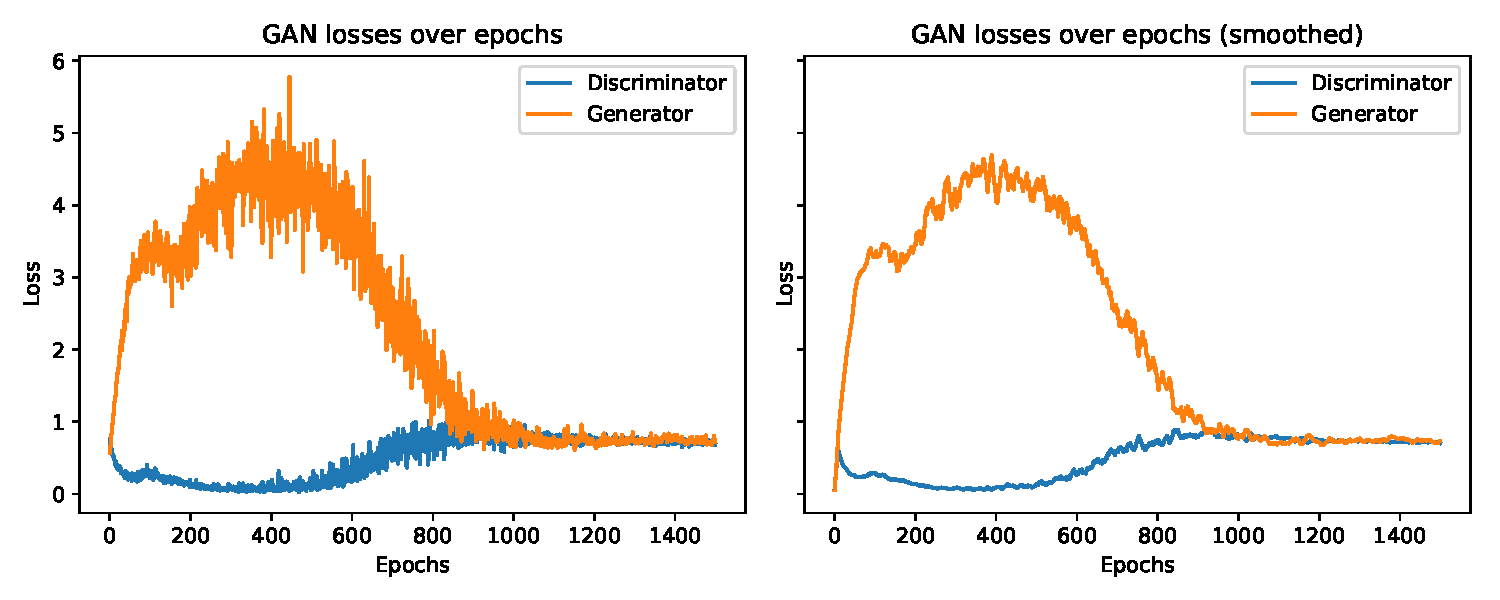
\includegraphics[width=15cm]{Figures/GAN_losses}
\caption{Generator and Discriminator losses over number of epochs}
\label{fig:GANLosses}
\end{figure}



\section{Verification}
It is useful to run a series of verification steps as a sanity check to the two neural networks that we just trained. While these do not give us a definite indication that the GAN was able to correctly capture and model the distribution in the training data, it is still useful to have a verification step in our pipeline.

\subsection{Generator}
Figure~\ref{fig:Qvalues} back in section~\ref{sec:analysisresults} showed the average intensity values of the Q-tables in the training test. As part of our verification process for the Generator, it is useful to show some samples of Q-tables that the neural network we just trained can produce.

In figure~\ref{fig:sampled_policies} we show sets of sampled Q-tables (16x4 matrices) from the Generator for different epochs, as we trained the GAN.

At epoch 0, we expect the Generator to produce random matrices, and that looks like the case. As we train the GAN, we produce Q-tables that will tend to fit within the initial distribution more and more.

It is still a fairly hard task to verify this visually. If we were training on the MNIST dataset of handwritten digits (0-9), we would have a clear visualisation of the digits evolving from random matrices to scribbles, to real-looking handwritten digits.

While we do not have a comparable, visual confirmation, we still notice a few things that are promising:
\begin{enumerate}
	\item In many sampled Q-tables, the second column or third column are the ones with the highest intensity in their row. This signifies that the policies our generator is producing tend to favour the actions of "going south" and "going east".
	\item Higher intensive values then accumulate in the bottom rows, since those are the closest to the goal state, and we expect the agent to have high probability of reaching the goal at that point.
	\item In all Q-tables, the last row (row 16), which corresponds to the goal state, has all its values set to 0 (that is because an episode ends when we reach the goal state, and we do not update the Q-table any further at that point).
\end{enumerate}

Another way we used to verify that the Generator has been trained well for our purposes is to use sample a Q-table and check that there is a map configuration in the training set that can be solved using the policy derived from the Q-table.

Indeed, we sampled 1,000 different Q-tables, and 826 of the policies derived from these Q-tables solve at least one task from the test set. We consider the task to be solved if it achieved at least 80\% of the score of the corresponding policy trained with Q-learning.

In comparison, sampling 1,000 random 16x4 matrices and deriving policies from these only yielded 23 solved tasks. These 23 tasks are the ones which have very few holes in the Frozen Lake environment, and in which it is therefore considerably easier to reach the goal state with random actions.

\begin{figure*}
\vskip 2mm
\centering{
\subfigure[\textbf{Epoch 0}]{
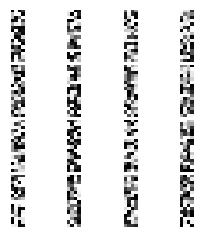
\includegraphics[width=5cm,height=4cm]{Figures/GeneratorPolicies/0000}}
\hskip 2cm
\subfigure[\textbf{Epoch 200}]{
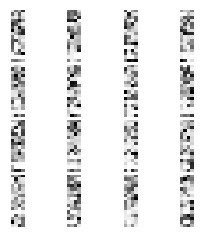
\includegraphics[width=5cm,height=4cm]{Figures/GeneratorPolicies/0200}}
\vskip 0.5cm
\subfigure[\textbf{Epoch 400}]{
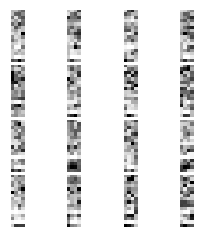
\includegraphics[width=5cm,height=4cm]{Figures/GeneratorPolicies/0400}}
\hskip 2cm
\subfigure[\textbf{Epoch 600}]{
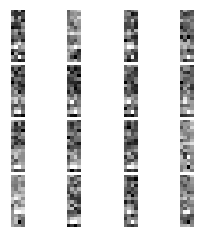
\includegraphics[width=5cm,height=4cm]{Figures/GeneratorPolicies/0600}}
\vskip 0.5cm
\subfigure[\textbf{Epoch 800}]{
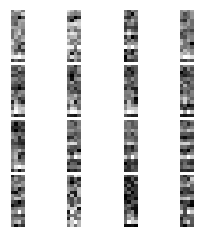
\includegraphics[width=5cm,height=4cm]{Figures/GeneratorPolicies/0800}}
\hskip 2cm
\subfigure[\textbf{Epoch 1000}]{
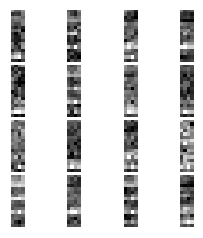
\includegraphics[width=5cm,height=4cm]{Figures/GeneratorPolicies/1000}}
\vskip 0.5cm
\subfigure[\textbf{Epoch 1200}]{
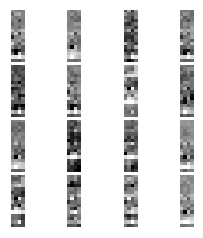
\includegraphics[width=5cm,height=4cm]{Figures/GeneratorPolicies/1200}}
\hskip 2cm
\subfigure[\textbf{Epoch 1500}]{
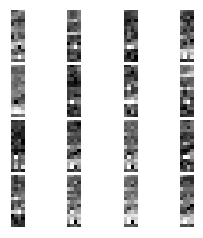
\includegraphics[width=5cm,height=4cm]{Figures/GeneratorPolicies/1500}}
}
\caption{Sampled policies produced by Generator over different epochs}
\label{fig:sampled_policies}
\vskip -2mm
\end{figure*}

\subsection{Discriminator}
In this subsection we present two sanity checks on the Discriminator network.

A first verification method is to run the Discriminator network with the Q-tables/policies in the test set. In other words, run a forward pass given the Q-tables in the test set as inputs.

We expect the Discriminator to label these as real Q-tables. Recall that the output of the Discriminator network is a single scalar value in $(0,1)$ representing the probability that the input policy is real or fake. The average output predicted value for the 765 policies in the test set is 0.79, indicating that the Discriminator correctly leans towards categorising these policies as being real.

% TODO: Plot?

As an additional check, we also retrain the test map configurations with Q-learning, but with half as many number of episodes (5,000 instead of 10,000). With fewer simulations and iterations in Q-learning, the policies that we train will yield lower average scores. We run these 1,000 of "half-trained" policies through the Discriminator once more. We obtain an average predicted score of 0.66. This is lower than the 0.79 we obtained with the policies in the test set, and it intuitively makes sense that we now obtain a lower average predicted value, since these "half-trained" policies do not fit the distribution of "fully-trained" policies in the training data.
Another set of sanity checks we conduct is to make sure that the Discriminator is not biased towards categorising any input as being real. We generate 1,000 random 16x4 matrices, and the average predicted output of the Discriminator is 0.008, which is a good sign that we have a healthy neural network.

In table~\ref{table:discrim_scores} we report the scores we obtained using these three different policies.

\begin{table}[H]
\centering
\begin{tabular}{@{}ll@{}}
\toprule
Policies                      & Mean Discriminator Score \\ \midrule
756 test policies             & 0.79                               \\
1,000 "half-trained" policies & 0.66                               \\
1,000 random policies         & 0.008                              \\ \bottomrule
\end{tabular}
\caption{Mean Predicted Discriminator Scores for different policies}
\label{table:discrim_scores}
\end{table}